%%%%%%%%%%%%%%%%%%%%%%%%%%%%%%%%%%%%%%%%%%%%%%%%%%%%%%%%%%%%%%%%%%%%%%%%%%%%%%%
%% SOCIOL 723 -- Social Statistics II
%% Week 2: Regression Inference and Robust Standard Errors
%% Wenhao Jiang, Duke University, Fall 2026
%%%%%%%%%%%%%%%%%%%%%%%%%%%%%%%%%%%%%%%%%%%%%%%%%%%%%%%%%%%%%%%%%%%%%%%%%%%%%%%

\documentclass[aspectratio=169,11pt,xcolor=dvipsnames]{beamer}
\mode<presentation>

%% ---- fonts: Latin Modern Roman (the LaTeX default), serif throughout -------
\usepackage[T1]{fontenc}
\usepackage{lmodern}
\usefonttheme{serif}
\renewcommand{\familydefault}{\rmdefault}

%% ---- packages --------------------------------------------------------------
\usepackage{amsmath,amsfonts,amssymb,bm}
\usepackage{graphicx}
\usepackage{booktabs}
\usepackage{tikz}
\usetikzlibrary{arrows.meta,positioning,calc}
\usepackage[english]{babel}

%% lightweight citation macros (beamer + natbib do not play well together)
\newcommand{\srcp}[1]{{\scriptsize\color{gray}(#1)}}   %% parenthetical
\newcommand{\srct}[1]{#1}                               %% inline / narrative

\DeclareMathOperator*{\argminop}{arg\,min}
\DeclareMathOperator*{\argmaxop}{arg\,max}
%% \limits forces the subscript underneath even in inline math
\newcommand{\argmin}{\argminop\limits}
\newcommand{\argmax}{\argmaxop\limits}
\DeclareMathOperator{\Cov}{Cov}
\DeclareMathOperator{\Var}{Var}
\DeclareMathOperator{\Corr}{Corr}
\DeclareMathOperator{\trace}{tr}
\DeclareMathOperator{\rank}{rank}
\DeclareMathOperator{\plim}{plim}
\newcommand{\indep}{\perp\!\!\!\perp}

%% ---- notation conventions (course-wide) ------------------------------------
%%  \E   population expectation (plain italic E)
%%  \En  sample / empirical expectation (blackboard-bold E)
%%  matrices and vectors are BOLD ITALIC via \bm
\newcommand{\E}{E}
\newcommand{\En}{\mathbb{E}_n}
\newcommand{\R}{\mathbb{R}}
\newcommand{\X}{\bm{X}}
\newcommand{\Y}{\bm{y}}
\newcommand{\Ix}{\bm{I}}
\newcommand{\zero}{\bm{0}}
\newcommand{\one}{\bm{1}}
\newcommand{\Pm}{\bm{P}}
\newcommand{\Mm}{\bm{M}}
\newcommand{\bhat}{\hat{\bm{\beta}}}
\newcommand{\ehat}{\hat{\bm{e}}}
\newcommand{\Om}{\bm{\Omega}}
\newcommand{\dto}{\overset{d}{\longrightarrow}}
\newcommand{\pto}{\overset{p}{\longrightarrow}}
\newcommand{\SE}{\mathrm{se}}

%% ---- theme -----------------------------------------------------------------
\usetheme{default}
%% thin single-line header: clickable section names, current one highlighted.
%% (miniframes is deliberately not used: one dot per slide wraps to 4 rows here)
\setbeamerfont{section in head/foot}{size=\tiny}
\setbeamertemplate{headline}{%
  \begin{beamercolorbox}[wd=\paperwidth,ht=2.4ex,dp=1.1ex,%
                         leftskip=.3cm,rightskip=.3cm]{section in head/foot}%
    \usebeamerfont{section in head/foot}%
    \insertsectionnavigationhorizontal{.94\paperwidth}{}{}%
  \end{beamercolorbox}%
}

\definecolor{dukeblue}{RGB}{1,33,105}
\definecolor{accent}{RGB}{200,78,0}
\definecolor{softgray}{RGB}{242,242,245}

\setbeamercolor{structure}{fg=dukeblue}
\setbeamercolor{frametitle}{fg=dukeblue,bg=white}
\setbeamercolor{section in head/foot}{fg=white,bg=dukeblue}
\setbeamercolor{section in head/foot shaded}{fg=white!50!dukeblue,bg=dukeblue}
\setbeamercolor{alerted text}{fg=accent}
\setbeamercolor{block title}{fg=white,bg=dukeblue}
\setbeamercolor{block body}{fg=black,bg=softgray}
\setbeamercolor{block title alerted}{fg=white,bg=accent}
\setbeamercolor{block body alerted}{fg=black,bg=softgray}

\setbeamertemplate{footline}[page number]
%% continued frames keep the SAME font size and spill onto a new slide
\setbeamertemplate{frametitle continuation}{\ifnum\insertcontinuationcount>1\normalfont\footnotesize\ (cont.)\fi}
\setbeamertemplate{navigation symbols}{}
\setbeamertemplate{itemize items}[circle]
\setbeamertemplate{blocks}[rounded][shadow=false]
\setbeamerfont{frametitle}{series=\bfseries}
\setbeamerfont{footnote}{size=\scriptsize}
\setbeamerfont{caption}{size=\footnotesize}
\setbeamertemplate{subsection in head/foot}{}
\setbeamertemplate{subsection in head/foot shaded}{}
\setbeamertemplate{caption}[numbered]

%% marker for material that is for understanding, not for examination
\newcommand{\adv}{\,\raisebox{0.6pt}{\textcolor{accent}{$\bigstar$}}}
%% marker for essential material every student must understand (examinable core)
\definecolor{corestar}{RGB}{0,83,155}
\newcommand{\core}{\,\raisebox{0.6pt}{\textcolor{corestar}{$\bigstar$}}}

\setbeamertemplate{section page}{%
  \begin{centering}\vfill
  {\usebeamercolor[fg]{structure}\Large\bfseries\insertsectionhead\par}
  \vskip4pt{\color{dukeblue}\rule{0.35\linewidth}{1pt}\par}
  \vfill\end{centering}}
\setbeamertemplate{subsection page}{%
  \begin{centering}\vfill
  {\usebeamercolor[fg]{structure}\large\bfseries\insertsubsectionhead\par}
  \vfill\end{centering}}

%% tighter vertical rhythm: math-heavy beamer frames otherwise overflow
\AtBeginDocument{%
  \setlength{\abovedisplayskip}{5pt}%
  \setlength{\belowdisplayskip}{5pt}%
  \setlength{\abovedisplayshortskip}{2pt}%
  \setlength{\belowdisplayshortskip}{3pt}%
}
\setbeamertemplate{frametitle}{%
  \vskip4pt\usebeamerfont{frametitle}\usebeamercolor[fg]{frametitle}%
  \insertframetitle\par\vskip2pt}
\setbeamersize{text margin left=0.75cm, text margin right=0.75cm}

%% ---- title -----------------------------------------------------------------
%% ---- title page: same face as the body (Latin Modern), larger and bold
\setbeamerfont{title}{size*={16}{19},series=\bfseries}
\setbeamerfont{subtitle}{size=\Large,series=\mdseries}
\setbeamerfont{author}{size=\large}
\setbeamerfont{date}{size=\large}
\title[SOCIOL 723]{SOCIOL 723: Social Statistics II\\[-2pt]}
\subtitle{Week 2, Regression Inference and Robust Standard Errors\\[-6pt]}
\author[Jiang]{Wenhao Jiang\vspace{-2.5em}}
\institute[Duke]{}
\titlegraphic{
\includegraphics[height=1.3cm]{../Misc/duke_logo.png}}
\date{Department of Sociology, Fall 2026}

\begin{document}

\begin{frame}[plain]
  \titlepage
\end{frame}

\begin{frame}{Today}
  \tableofcontents
  \vskip6pt
  {\footnotesize \core{} $=$ essential, you must understand this \quad\quad \adv{} $=$ for understanding, not examined}
\end{frame}

\begin{frame}{Where We Left Off}
Last week, for the bivariate model $Y_i = \beta_0 + \beta_1X_i + \epsilon_i$:
\begin{align*}
  \hat\beta_1 - \beta_1
  = \frac{\sum_i (X_i - \bar X)\,\epsilon_i}{\sum_i (X_i-\bar X)^2},
  \qquad
  \Var(\hat\beta_1\mid X)
  = \frac{\sum_i (X_i-\bar X)^2\,\Var(\epsilon_i\mid X)}
         {\big[\sum_i (X_i - \bar X)^2\big]^2} ,
\end{align*}
which collapses to $\sigma^2 / \sum_i (X_i-\bar X)^2$ only if
$\Var(\epsilon_i\mid X)$ is the same for every $i$.
\vskip4pt
\begin{block}{Today's agenda}
\begin{enumerate}\itemsep1pt
  \item What is the sampling distribution of $\hat\beta_1$ as $n$ grows?
  \item How do we turn a standard error into a test and a confidence
        interval?
  \item What if $\Var(\epsilon_i\mid X)$ is \emph{not} constant?
        (Heteroskedasticity, then clustering.)
  \item The bootstrap as a general-purpose alternative.
  \item \alert{What robust standard errors can and cannot fix.}
\end{enumerate}
\end{block}
\end{frame}

\begin{frame}{Reminder: the Two-Star Convention}
\begin{alertblock}{}
Frames marked \core{} are \textbf{essential}: problem sets and exams draw on
them directly. Frames marked \adv{} are here for \emph{understanding}, not for
evaluation: matrix derivations, asymptotic arguments, and the general formulas
you will meet in the literature.
\end{alertblock}
\vskip6pt
\begin{itemize}\itemsep4pt
  \item Examinable this week: the scalar variance formula and where it comes from;
        what heteroskedasticity and clustering \emph{are} and why they matter;
        how to read and choose a standard error; what a bootstrap does; and the
        list of problems robust standard errors do not solve.
  \item Every standard error in this course starts from the variance of a
        weighted sum of errors. HC estimators estimate the individual
        \emph{variance} terms; cluster-robust estimators also estimate the
        within-cluster \emph{covariance} terms. Hold on to that sentence.
\end{itemize}
\end{frame}

%%%%%%%%%%%%%%%%%%%%%%%%%%%%%%%%%%%%%%%%%%%%%%%%%%%%%%%%%%%%%%%%%%%%%%%%%%%%%%%
\section[Sampling Distribution]{The Sampling Distribution of OLS}
%%%%%%%%%%%%%%%%%%%%%%%%%%%%%%%%%%%%%%%%%%%%%%%%%%%%%%%%%%%%%%%%%%%%%%%%%%%%%%%
\begin{frame}\sectionpage\end{frame}

\begin{frame}{The Question, in Plain Words\core}
Last week we computed $\hat\beta_1 = 0.119$: one more year of schooling goes
with about $12\%$ higher earnings in our sample of $3{,}509$ people.
\vskip3pt
\begin{itemize}\itemsep3pt
  \item The GSS could just as easily have interviewed a \emph{different}
        3{,}509 people. That sample would have produced a different number,
        perhaps $0.112$, perhaps $0.127$.
  \item So $0.119$ is one draw from a lottery. Before treating it as evidence
        about the population, we need to know how much it moves from draw to
        draw.
  \item The \alert{standard error} is exactly that: the give-or-take attached
        to the estimate. Formally, it is (an estimate of) the standard
        deviation of $\hat\beta_1$ across hypothetical repeated samples.
\end{itemize}
\vskip3pt
\begin{block}{This week in one sentence}
Everything called ``statistical inference'', standard errors, $t$-statistics,
$p$-values, confidence intervals, is machinery for learning that give-or-take
number from the single sample we actually have.
\end{block}
\end{frame}

\begin{frame}{What a Sampling Distribution Is\core}
$\hat\beta_1$ is a number computed from \emph{your} sample. Had you drawn a
different sample from the same population, you would have got a different number.
\vskip4pt
\begin{block}{The thought experiment}
Imagine drawing sample after sample from the population and computing
$\hat\beta_1$ each time. The histogram of those numbers is the \alert{sampling
distribution}. Where it is centered tells you about bias; how wide it is is
the true sampling standard deviation, and the \emph{standard error} is our
estimate of that width.
\end{block}
\vskip4pt
\begin{itemize}\itemsep3pt
  \item You only ever see one draw. Everything in this lecture is about inferring
        the shape of that histogram from a single sample.
  \item In lab we run the experiment by simulation, which is the fastest way to
        make the idea concrete.
\end{itemize}
\end{frame}

\begin{frame}{Two Theorems We Lean On All Semester\core}
Both are statements about what happens to a \emph{sample average} as $n$ grows.
\vskip2pt
\begin{block}{Law of large numbers (LLN)}
The average of $n$ independent draws settles down on the population mean:
$\frac1n\sum_i Z_i \pto \E[Z]$ (read $\pto$ as ``settles down on''). Flip a fair coin 10 times and the share of
heads could be anything; flip it 10{,}000 times and it sits within a whisker
of $0.5$.
\end{block}
\vskip2pt
\begin{block}{Central limit theorem (CLT)}
For an average of \emph{independent} draws, the \emph{shape} of the wobble
around the truth becomes a bell curve, $\sqrt n\,(\bar Z - \E[Z]) \dto
\mathcal N\big(0, \Var(Z)\big)$ (read $\dto$ as ``the distribution
approaches''), \alert{whatever the distribution of $Z$ itself}, so long as
its variance is finite.
\end{block}
\vskip2pt
Why we care: $\hat\beta_1$ is built from sample averages, so the LLN gives
consistency and the CLT approximate normality. Thursday's lab watches the
bell curve emerge.
\end{frame}

\begin{frame}{The Sampling Distribution of $\hat\beta_1$, as $n$ Grows}
The big picture: \alert{keep drawing samples from the population; as $n$
grows, we will show that $\hat\beta_1$'s sampling behaviour approximates a
normal distribution}, without ever assuming the errors are normal (A6):
\begin{align*}
  \hat\beta_1 - \beta_1 = \frac{\frac1n\sum_i (X_i-\bar X)\epsilon_i}
                               {\frac1n\sum_i (X_i-\bar X)^2} .
\end{align*}
A normal is pinned down by its \emph{mean} and \emph{variance}, so the work
here is to find both, and let the CLT supply the \emph{shape}.
\vskip2pt
The plan:
\begin{enumerate}\itemsep0pt
  \item The denominator converges to a constant (LLN).
  \item The numerator, magnified by $\sqrt n$, converges to a normal
        distribution with mean $0$ (CLT) under strict exogeneity (A4: $\E[\epsilon_i \mid X] = 0 ]$).
  \item A normal distribution divided by a settled constant is still normal.
\end{enumerate}
\end{frame}

\begin{frame}{Step 1: The Denominator Settles (LLN)}
The denominator is the sample variance of $X$. By the law of large numbers
\begin{align*}
  \bar X \ &\pto\ \E[X] = \mu_X , \\
  \frac1n\sum_i (X_i - \bar X)^2 \ &\pto\ \E[ (X_i - \mu_X)^2 ] = \Var(X_i)
\end{align*}
\begin{itemize}
      \item It settles on the population variance, a \emph{positive constant}.
      \item As $n \to \infty$, the observed $X$'s approach, in aggregate, the
        population distribution of $X$.
      \item From here on we may treat the denominator as the constant $\Var(X_i)$. Every
remaining question is about the numerator, whose terms we may likewise write
with $\mu_X$ in place of $\bar X$: it is the average of the
$(X_i - \mu_X)\,\epsilon_i$.
\end{itemize} 
\end{frame}

\begin{frame}{Step 2: The Numerator's Mean}
The numerator averages the identically distributed terms
$(X_i - \mu_X)\,\epsilon_i$, so its mean is the terms' common mean. Compute it:
\begin{align*}
  \E\big[(X_i - \mu_X)\,\epsilon_i\big]
  &= \E\Big[\,\E\big[(X_i - \mu_X)\,\epsilon_i \mid X_i\big]\,\Big]
    && \text{\footnotesize iterated expectations} \\
  &= \E\big[(X_i - \mu_X)\,\E[\epsilon_i \mid X_i]\big]
    && \text{\footnotesize given $X_i$, $(X_i-\mu_X)$ is fixed} \\
  &= \E\big[(X_i - \mu_X)\cdot 0\big] \;=\; 0
    && \text{\footnotesize A4: } \E[\epsilon_i \mid X_i] = 0
\end{align*}
\begin{itemize}\itemsep3pt
  \item By the LLN the numerator settles on this mean, $0$, so
        $\hat\beta_1 - \beta_1 \pto 0/\Var(X_i) = 0$: \alert{consistency}.
        As sample approaches population, $\hat\beta_1$ nails $\beta_1$.
  \item But a mean says nothing about \emph{spread}, and spread is what a
        standard error measures. Next: the variance.
\end{itemize}
\end{frame}

\begin{frame}{Step 3: The Numerator's Variance}
Take $n = 3$: the numerator averages the three terms
$(X_i-\mu_X)\,\epsilon_i$. The variance of a sum is every term's variance
plus a covariance for every pair:
\begingroup\small
\setlength{\abovedisplayskip}{3pt}\setlength{\belowdisplayskip}{3pt}
\begin{align*}
  \Var(\text{numerator})
  = \tfrac19\Big[
  &\underbrace{\Var\big((X_1-\mu_X)\epsilon_1\big)
    + \Var\big((X_2-\mu_X)\epsilon_2\big)
    + \Var\big((X_3-\mu_X)\epsilon_3\big)}
    _{\text{one variance per draw}} \\
  &+ \underbrace{2\Cov\big((X_1-\mu_X)\epsilon_1,\ (X_2-\mu_X)\epsilon_2\big)
    + \cdots}
    _{\text{one covariance per pair; $3$ pairs}}\ \Big]
\end{align*}
\endgroup
\vskip-2pt
\begin{itemize}\itemsep0pt
  \item A2 kills every covariance: draws are \emph{independent},
        so each $\Cov$ is $0$. Clustering breaks exactly this step.
  \item Merging the remaining variance terms, with $n$ draws,
        $\Var\big((X_i-\mu_X)\epsilon_i\big)/n$.
  \item The spread shrinks like $1/\sqrt n$: \alert{magnify by $\sqrt n$} to
        hold it steady. That is where the $\sqrt n$ comes from.
\end{itemize}
\end{frame}

\begin{frame}{Step 4: The CLT Adds the Shape}
The magnified numerator has mean $0$ and variance
$\Var\big((X_i-\mu_X)\epsilon_i\big)$; the CLT adds the missing \emph{shape}.
Divide by the settled denominator:
\begingroup
\setlength{\abovedisplayskip}{2pt}\setlength{\belowdisplayskip}{2pt}
\begin{align*}
  \sqrt n\,\big(\hat\beta_1 - \beta_1\big)
  = \frac{\overbrace{\sqrt n\cdot\tfrac1n\sum_i (X_i-\bar X)\,\epsilon_i}
          ^{\ \dto\ \mathcal N\left(0,\ \Var\left((X_i-\mu_X)\epsilon_i\right)\right)}}
         {\underbrace{\tfrac1n\sum_i (X_i-\bar X)^2}_{\ \pto\ \Var(X_i)}}
  \;\dto\;
  \mathcal N\big(0,\ V\big) ,
  \quad
  V = \frac{\Var\big((X_i-\mu_X)\epsilon_i\big)}{\big[\Var(X_i)\big]^2} .
\end{align*}
\endgroup
\vskip-2pt
\begin{itemize}\itemsep0pt
  \item Under A5, homoskedasticity, $\Var(\epsilon_i \mid X_i) = \sigma^2$:
        the error variance is the same number at every value of $X$. The
        numerator of $V$ then collapses and $V = \sigma^2/\Var(X_i)$, the
        familiar formula: next frame, slowly.
  \item Without A5, \alert{estimating $V$ is this lecture's entire subject}.
\end{itemize}
\end{frame}

\begin{frame}{Under A4 and A5, the Meat Collapses}
The meat is a mean square around the unconditional mean, so A4 first
certifies that mean is zero; then A5 collapses it:
\begin{align*}
  \E\big[(X_i-\mu_X)^2\,\epsilon_i^2\big]
  &= \E\Big[\,\E\big[(X_i-\mu_X)^2\,\epsilon_i^2 \mid X_i\big]\,\Big]
    && \text{\footnotesize iterated expectations} \\
  &= \E\big[(X_i-\mu_X)^2\,\E[\epsilon_i^2 \mid X_i]\big]
    && \text{\footnotesize given $X_i$, $(X_i-\mu_X)^2$ is fixed} \\
  &= \E\big[(X_i-\mu_X)^2\,\sigma^2\big]
    && \text{\footnotesize A4 + A5: $\E[\epsilon_i^2 \mid X_i] = \sigma^2$} \\
  &= \sigma^2\,\E\big[(X_i-\mu_X)^2\big] = \sigma^2\,\Var(X_i)
    && \text{\footnotesize $\sigma^2$ is one number: pull it out}
\end{align*}
So $V = \sigma^2\Var(X_i)\big/[\Var(X_i)]^2 = \sigma^2/\Var(X_i)$: the same
answer as Week 1.
\end{frame}

%%%%%%%%%%%%%%%%%%%%%%%%%%%%%%%%%%%%%%%%%%%%%%%%%%%%%%%%%%%%%%%%%%%%%%%%%%%%%%%
\section[Testing]{Hypothesis Testing}
%%%%%%%%%%%%%%%%%%%%%%%%%%%%%%%%%%%%%%%%%%%%%%%%%%%%%%%%%%%%%%%%%%%%%%%%%%%%%%%
\begin{frame}\sectionpage\end{frame}

\begin{frame}{The Vocabulary, Pinned Down\core}
You met these words in \textit{Social Statistics I}; now they have foundations.
\begin{itemize}\itemsep3pt
  \item A \textbf{null hypothesis} $H_0$ is a specific claim about a population
        quantity, e.g.\ $\beta_1 = 0$: schooling and earnings are unrelated.
  \item A \textbf{test statistic} measures the distance between estimate and
        null \emph{in standard-error units}: $t = (\hat\beta_1 - 0)/
        \mathrm{se}(\hat\beta_1)$. Big distance, implausible null.
  \item The \textbf{$p$-value}: \emph{if} $H_0$ were true, how often would
        sampling noise alone produce a $t$ this large? It is a statement about
        the data under the null, \alert{not} the probability the null is true.
  \item A \textbf{95\% confidence interval} collects every null value the data
        cannot reject; across repeated samples, intervals built this way cover
        the truth 95\% of the time. \emph{This} interval either does or does
        not; the 95\% describes the procedure.
\end{itemize}
\end{frame}

\begin{frame}{Testing a Single Coefficient\core}
To test $H_0: \beta_j = \beta_j^0$, compare
\begin{align*}
  t = \frac{\hat\beta_j - \beta_j^0}{\SE(\hat\beta_j)}
\end{align*}
against $t_{n-k}$ critical values; a $95\%$ confidence interval is
$\hat\beta_j \pm t_{0.975,\,n-k}\,\SE(\hat\beta_j)$.
\vskip6pt
\begin{itemize}\itemsep4pt
  \item By the last section, $t$ is approximately $\mathcal N(0,1)$ for
        large $n$, and $t_{n-k}$ merges into that same curve (the critical
        values differ by under $2\%$ once $n-k > 100$); under the classical
        assumption of normal errors, $t_{n-k}$ is even exact at any $n$,
        which is where the convention comes from. This is why regression
        output reports $t_{n-k}$; clustered data will later change the
        right degrees of freedom.
  \item \alert{Everything depends on whether $\SE$ is right.} A $t$ of 3.0
        computed from a standard error that is half of what it should be is
        really a $t$ of 1.5.
\end{itemize}
\end{frame}

%%%%%%%%%%%%%%%%%%%%%%%%%%%%%%%%%%%%%%%%%%%%%%%%%%%%%%%%%%%%%%%%%%%%%%%%%%%%%%%
\section[Heteroskedasticity]{Heteroskedasticity and Robust Standard Errors}
%%%%%%%%%%%%%%%%%%%%%%%%%%%%%%%%%%%%%%%%%%%%%%%%%%%%%%%%%%%%%%%%%%%%%%%%%%%%%%%
\begin{frame}\sectionpage\end{frame}

\begin{frame}{What Heteroskedasticity Is\core}
Week 1's A5 had \emph{two} parts: constant variance, and zero covariance
across observations. This section drops the first while keeping the second;
the clustering section then drops the second.
\textbf{Homoskedasticity} says $\Var(\epsilon_i\mid X_i) = \sigma^2$: the
spread of the outcome around the line is the same everywhere.
\vskip2pt
\begin{center}
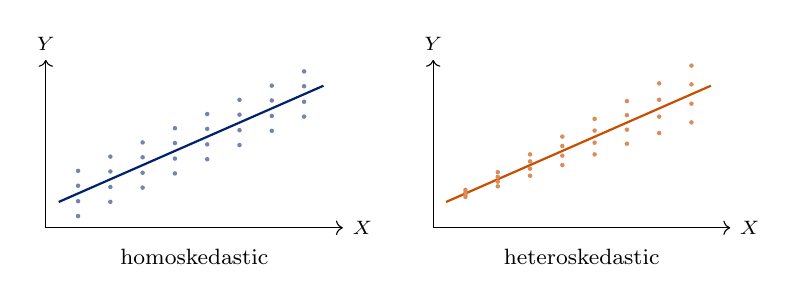
\begin{tikzpicture}[scale=0.82]
  \begin{scope}
    \draw[->] (0,0) -- (4.6,0) node[right]{\scriptsize $X$};
    \draw[->] (0,0) -- (0,2.6) node[above]{\scriptsize $Y$};
    \draw[dukeblue,thick] (0.2,0.4) -- (4.3,2.2);
    \foreach \x in {0.5,1.0,...,4.2} {
      \foreach \d in {-0.35,-0.12,0.12,0.35} {
        \fill[dukeblue!55] (\x, {0.4+(\x-0.2)*0.44+\d}) circle (0.035);}}
    \node at (2.3,-0.45) {\footnotesize homoskedastic};
  \end{scope}
  \begin{scope}[xshift=6cm]
    \draw[->] (0,0) -- (4.6,0) node[right]{\scriptsize $X$};
    \draw[->] (0,0) -- (0,2.6) node[above]{\scriptsize $Y$};
    \draw[accent,thick] (0.2,0.4) -- (4.3,2.2);
    \foreach \x in {0.5,1.0,...,4.2} {
      \foreach \d in {-1,-0.34,0.34,1} {
        \fill[accent!65] (\x, {0.4+(\x-0.2)*0.44+\d*0.11*\x}) circle (0.035);}}
    \node at (2.3,-0.45) {\footnotesize heteroskedastic};
  \end{scope}
\end{tikzpicture}
\end{center}
\vskip2pt
Under exogeneity, both lines are estimated without bias: heteroskedasticity by
itself does not bias $\hat\beta$. Only the \emph{uncertainty} about them differs,
and only the right-hand panel needs a different formula.
\end{frame}

\begin{frame}{Heteroskedasticity Is the Norm}
\begin{itemize}\itemsep4pt
  \item Earnings dispersion rises steeply with education and experience: at 8
        years of schooling almost everyone earns a modest wage; at 20 years the
        range is enormous.
  \item Group-level outcomes built from different numbers of individuals, a
        county mean over 50 people is noisier than one over 50{,}000.
  \item Binary outcomes: $\Var(Y_i\mid X_i) = p(X_i)(1-p(X_i))$ is
        \emph{necessarily} heteroskedastic, so the linear probability model always
        violates A5.
\end{itemize}
\vskip3pt
\begin{block}{What it does and does not do}
\textbf{Does not}: bias $\hat\beta$ or break consistency (given A4 and
random sampling). \\
\textbf{Does}: invalidate the standard errors your software prints by default, so
$t$-statistics, $p$-values and confidence intervals are wrong.
\end{block}
\end{frame}

\begin{frame}{The Scalar Sandwich\core}
The last section already handed us the bell's variance, built from population moments:
\begin{align*}
  V = \frac{\E\big[(X_i-\mu_X)^2\,\epsilon_i^2\big]}{\big[\Var(X_i)\big]^2}
    = \frac{\text{``meat''}}{\text{``bread''}^2} .
\end{align*}
\begin{itemize}\itemsep3pt
  \item The meat is a \alert{$(X_i-\mu_X)^2$-weighted average of the squared
        errors}: errors sitting far from the mean of $X$ count the most.
  \item Under A5 the squared error averages to $\sigma^2$ at every value of
        $X$, so the meat factors into $\sigma^2\,\Var(X_i)$ and
        $V = \sigma^2/\Var(X_i)$: \alert{the classical formula is the A5
        special case.}
  \item Without A5 nothing factors, and the classical formula is simply
        wrong. But every piece of $V$ is a population mean, and
        \alert{sample averages estimate population means}. Next frame.
\end{itemize}
\end{frame}

\begin{frame}{White's Estimator, in Scalar Form\core}
Estimate each population mean by its sample counterpart, with residuals
standing in for the unobservable errors: writing $d_i \equiv X_i - \bar X$,
the bread $\Var(X_i)$ becomes $\frac1n\sum_i d_i^2$ and the meat
$\E[(X_i-\mu_X)^2\epsilon_i^2]$ becomes $\frac1n\sum_i d_i^2\,\hat e_i^2$.
The squared standard error of $\hat\beta_1$ is this estimate of $V$,
divided by $n$; the $1/n$'s cancel into
\begin{align*}
  \boxed{\;
  \hat{V}_{\text{HC0}}(\hat\beta_1)
  = \frac{\sum_i d_i^2\,\hat e_i^2}{\big(\sum_i d_i^2\big)^2} \;}
  \qquad
  \text{versus}\qquad
  \hat{V}_{\text{classical}}(\hat\beta_1) = \frac{s^2}{\sum_i d_i^2} .
\end{align*}
\begin{itemize}\itemsep2pt
  \item That is the whole of ``heteroskedasticity-robust'' and
        ``(Eicker--)Huber--White'' (\srct{White 1980}); \texttt{Stata}'s
        \texttt{robust} adds HC1 scaling, next frame.
  \item With controls, replace $d_i$ by Week 1's FWL residual $\tilde d_i$:
        $\hat V(\hat\beta_j) = \sum_i \tilde d_i^{\,2}\hat e_i^2 \big/
        \big(\sum_i \tilde d_i^{\,2}\big)^2$: same formula, residualized weights.
  \item The classical formula pools \emph{one} $s^2$; the robust one lets
        each observation carry its own $\hat e_i^2$.
\end{itemize}
\end{frame}

\begin{frame}{The General Statement\adv}
For the full coefficient vector, with $X_i$ now the \emph{vector} of
observation $i$'s regressors and sample averages written as $\En$:
\begin{align*}
  \bhat - \bm\beta
  = \big(\En[X_iX_i']\big)^{-1}\En[X_i\epsilon_i] ,
  \qquad
  \En[X_iX_i'] = \tfrac1n\sum_i X_iX_i' = \tfrac1n \X'\X ,
\end{align*}
so this is Thursday's $(\X'\X)^{-1}\X'\bm\epsilon$, each factor scaled by
$\tfrac1n$. The LLN gives $\En[X_iX_i'] \pto \E[X_iX_i'] \equiv \bm{Q}$ and
$\En[X_i\epsilon_i]\pto \zero$, so $\bhat \pto \bm\beta$ (\emph{consistency}).
Multiplying by $\sqrt n$ and applying the CLT to the second factor,
\begin{align*}
  \boxed{\;\sqrt n(\bhat-\bm\beta) \dto
  \mathcal N\Big(\zero,\; \bm{Q}^{-1}\Om\bm{Q}^{-1}\Big)\;},
  \qquad \Om = \E[\epsilon_i^2 X_iX_i'] .
\end{align*}
\vskip2pt
Note what is \emph{not} assumed: no normality, no homoskedasticity.
\end{frame}

\begin{frame}{Reading the ``Sandwich''\adv}
\begingroup
\setlength{\abovedisplayskip}{2pt}\setlength{\belowdisplayskip}{2pt}
\begin{align*}
  \bm{V} = \underbrace{\bm{Q}^{-1}}_{\text{bread}}\;
           \underbrace{\Om}_{\text{meat}}\;
           \underbrace{\bm{Q}^{-1}}_{\text{bread}},
  \qquad
  \bm Q = \E[X_iX_i'],\quad \Om = \E[\epsilon_i^2X_iX_i'] .
\end{align*}
Estimated by sample analogues, the $1/n$'s cancel into Thursday's matrices:
\begin{align*}
  \widehat{\Var}_{\text{HC0}}(\bhat)
  = (\X'\X)^{-1}\Big(\sum_i \hat e_i^2\, X_iX_i'\Big)(\X'\X)^{-1} :
\end{align*}
what \texttt{vcovHC} computes; the clustered version later swaps only the
middle sum.
\endgroup
\begin{itemize}\itemsep1pt
  \item The \textbf{bread} depends only on the regressors; the \textbf{meat}
        is where every assumption about the errors lives. Classical, robust,
        clustered, and HAC differ \alert{only} in the meat.
  \item If $\E[\epsilon_i^2\mid X_i] = \sigma^2$, the meat is
        $\sigma^2\bm Q$ and $\bm V = \sigma^2\bm Q^{-1}$: the classical
        formula.
\end{itemize}
\vskip3pt
\begin{alertblock}{The organizing idea for the estimator}
Keep the estimator $\hat\beta$ and the bread; change only the meat.
\end{alertblock}
\end{frame}

\begin{frame}{From Scalar to Matrix: the Dictionary\adv}
One change of meaning: $X_i$ now denotes the \emph{vector} of observation
$i$'s regressors, in the bivariate case $X_i = (1,\ X_i)'$. Then
\begin{align*}
  X_iX_i' = \begin{pmatrix} 1 & X_i \\ X_i & X_i^2 \end{pmatrix},
  \qquad
  X_i\epsilon_i = \begin{pmatrix} \epsilon_i \\ X_i\epsilon_i \end{pmatrix},
\end{align*}
and their sample averages stack the scalar sums you have used all lecture:
\begin{align*}
  \En[X_iX_i'] =
  \begin{pmatrix} 1 & \bar X \\ \bar X & \tfrac1n\sum_i X_i^2 \end{pmatrix},
  \qquad
  \En[X_i\epsilon_i] =
  \begin{pmatrix} \bar\epsilon \\ \tfrac1n\sum_i X_i\epsilon_i \end{pmatrix}.
\end{align*}
\begin{itemize}\itemsep2pt
  \item Population versions: $\bm Q = \E[X_iX_i']$ and the meat
        $\Om = \E[\epsilon_i^2X_iX_i']$, which stacks
        $\E[\epsilon_i^2]$, $\E[X_i\epsilon_i^2]$, $\E[X_i^2\epsilon_i^2]$.
  \item These are the objects inside the sandwich you just saw. The next
        frames multiply it out until the slope's entry is \emph{exactly} the
        scalar $V$.
\end{itemize}
\end{frame}

\begin{frame}{The Dictionary, Cashed: Multiply the Sandwich Out\adv}
Every symbol below is a population \emph{number}. Abbreviate
$v = \Var(X_i)$, $q = \E[X_i^2]$, and the meat's three entries
$a = \E[\epsilon_i^2]$, $b = \E[X_i\epsilon_i^2]$,
$c = \E[X_i^2\epsilon_i^2]$. The ingredients ($\bm Q^{-1}$ by the
$2\times2$ inverse, $\det\bm Q = q - \mu_X^2 = v$):
\begin{align*}
  \bm Q^{-1} = \frac1v
  \begin{pmatrix} q & -\mu_X \\ -\mu_X & 1 \end{pmatrix},
  \qquad
  \Om = \begin{pmatrix} a & b \\ b & c \end{pmatrix} .
\end{align*}
First multiplication, plain row-times-column arithmetic:
\begin{align*}
  \Om\bm Q^{-1}
  = \frac1v
  \begin{pmatrix}
    aq - b\mu_X & \ b - a\mu_X \\
    bq - c\mu_X & \ c - b\mu_X
  \end{pmatrix} .
\end{align*}
One more multiplication by $\bm Q^{-1}$ from the left: next frame.
\end{frame}

\begin{frame}{The Final $2\times2$ Matrix\adv}
Multiply again, row times column; for instance the bottom-right entry is
$(-\mu_X)(b - a\mu_X) + 1\cdot(c - b\mu_X) = a\mu_X^2 - 2b\mu_X + c$.
Collecting all four entries:
\begin{align*}
  \bm Q^{-1}\Om\bm Q^{-1}
  = \frac{1}{v^2}
  \begin{pmatrix}
    aq^2 - 2bq\mu_X + c\mu_X^2 & \ b(q+\mu_X^2) - \mu_X(aq+c) \\[2pt]
    b(q+\mu_X^2) - \mu_X(aq+c) & \ \alert{a\mu_X^2 - 2b\mu_X + c}
  \end{pmatrix} .
\end{align*}
The highlighted slope entry, with $a,b,c$ substituted back:
\begin{align*}
  a\mu_X^2 - 2b\mu_X + c
  = \E\big[\mu_X^2\epsilon_i^2 - 2\mu_X X_i\epsilon_i^2
    + X_i^2\epsilon_i^2\big]
  = \E\big[(X_i - \mu_X)^2\epsilon_i^2\big] ,
\end{align*}
so the $(2,2)$ entry is $\E[(X_i-\mu_X)^2\epsilon_i^2]/v^2 = V$: the scalar
sandwich, recovered.
\vskip2pt
{\footnotesize Reading the rest: the diagonal holds the intercept's and the
slope's variances, the off-diagonal their covariance.}
\end{frame}

\begin{frame}{Why the Squared Residuals Are Systematically Too Small}
The meat is estimated by an average, and averages forgive noise: each
$d_i^2\hat e_i^2$ may be a poor estimate of its own term, yet the mean still
finds the target. \alert{What an average does not forgive is an error shared
by every term} -- and the squared residuals carry one.
\begin{itemize}\itemsep4pt
  \item OLS chooses the line that makes the residuals as small as possible,
        so it partly fits the noise itself: residuals run systematically
        \emph{smaller} than the errors they stand in for.
  \item The exact bookkeeping (under A5, for clean arithmetic):
        $\E[\hat e_i^2 \mid X] = \sigma^2(1 - h_{ii})$, where the
        \alert{leverage} $h_{ii} = \tfrac1n + d_i^2\big/\sum_j d_j^2$
        measures how unusual $X_i$ is.
  \item So every $\hat e_i^2$ is deflated, and most at \emph{high-leverage}
        observations, exactly the ones the meat weights most heavily. The
        meat estimate, hence HC0, is \alert{biased down in small samples}.
  \item As $n$ grows, $h_{ii} \to 0$ and the deflation vanishes: a purely
        finite-sample issue. The target is still only the meat; the fixes
        just undo a known bias in its ingredients.
\end{itemize}
\end{frame}

\begin{frame}{Where $\sigma^2(1-h_{ii})$ Comes From\adv}
Write the residual in terms of the errors, step by step:
\begingroup
\setlength{\abovedisplayskip}{3pt}\setlength{\belowdisplayskip}{3pt}
\begin{align*}
  \hat e_i &= Y_i - \hat\beta_0 - \hat\beta_1 X_i
    && \text{\footnotesize definition} \\
  &= \epsilon_i - \bar\epsilon - (\hat\beta_1 - \beta_1)\,d_i
    && \text{\footnotesize sub $Y_i = \beta_0+\beta_1X_i+\epsilon_i$,
       $\hat\beta_0 = \bar Y - \hat\beta_1\bar X$} \\
  &= \epsilon_i - \bar\epsilon
     - d_i\,\frac{\sum_j d_j\epsilon_j}{\sum_j d_j^2}
   = \epsilon_i - \sum_j w_{ij}\,\epsilon_j
    && \text{\footnotesize Week 1: $\hat\beta_1-\beta_1 =
       \textstyle\sum_j d_j\epsilon_j/\sum_j d_j^2$}
\end{align*}
\endgroup
with $w_{ij} = \tfrac1n + d_i d_j\big/\sum_k d_k^2$: the fitted line absorbs
a weighted share of \emph{every} error, with weight $w_{ii} = h_{ii}$ on
observation $i$'s own. Under A5 and uncorrelated errors,
\begin{align*}
  \E[\hat e_i^2 \mid X]
  = \sigma^2\Big(1 - 2h_{ii} + \sum_j w_{ij}^2\Big)
  = \sigma^2\,(1-h_{ii}),
\end{align*}
because $\sum_j w_{ij}^2 = h_{ii}$ (expand the square; $\sum_j d_j = 0$).
\vskip1pt
{\footnotesize Reading: observation $i$ pulls the line toward itself with
strength $h_{ii}$; the residual keeps the $(1-h_{ii})$ share. At $n=2$,
$h_{ii}=1$: the line passes through both points and both residuals are
exactly zero.}
\end{frame}

\begin{frame}{Finite-Sample Corrections: HC0--HC3\core}
Every $\hat e_i^2$ is deflated by its leverage. The corrections rescale each
squared residual before it enters the meat, undoing the deflation (factors
motivated by the homoskedastic benchmark, used regardless):
\begin{center}\small
\renewcommand{\arraystretch}{1.15}
\begin{tabular}{lll}
\toprule
& Meat uses & Comment \\
\midrule
HC0 & $\hat e_i^2$ & White's original; anticonservative when $n$ is small \\
HC1 & $\frac{n}{n-k}\hat e_i^2$ & simple d.f.\ correction; \texttt{Stata}'s
      \texttt{robust} default \\
HC2 & $\dfrac{\hat e_i^2}{1-h_{ii}}$ & exact at the homoskedastic benchmark \\
HC3 & $\dfrac{\hat e_i^2}{(1-h_{ii})^2}$ & jackknife-like; \alert{recommended default} \\
\bottomrule
\end{tabular}
\end{center}
\vskip2pt
{\footnotesize All four are consistent under any heteroskedasticity pattern
and coincide as $n \to \infty$. \srct{MacKinnon and White (1985)},
\srct{Long and Ervin (2000)}: with $n < 250$ or high leverage, use
\textbf{HC3}.}
\end{frame}

\begin{frame}{How Much Does It Matter?}
\begin{itemize}\itemsep4pt
  \item Robust standard errors can be \emph{larger or smaller} than classical
        ones. There is no general direction.
  \item The difference is driven by whether the error variance happens to be
        large where $X$ is extreme. In our GSS earnings regression it is modest:
        $\SE(\hat\beta_{\texttt{educ}})$ goes from $0.00510$ (classical) to
        $0.00547$ (HC0) to $0.00549$ (HC3), about $7\%$.
  \item With a skewed or sparse regressor, a rare binary treatment, a
        long-tailed count; the difference can be a factor of two.
  \item \alert{Clustering, by contrast, routinely changes standard errors by
        factors of three to ten.} In most sociological data that is the bigger
        issue.
\end{itemize}
\end{frame}

\begin{frame}{Should You \emph{Test} for Heteroskedasticity?}
Classical tests exist: Breusch--Pagan, White.
\vskip3pt
\begin{alertblock}{Recommendation: no}
Do not pre-test and then choose. Just report robust standard errors.
\end{alertblock}
\begin{itemize}\itemsep3pt
  \item A pre-test makes your final inference conditional on the pre-test outcome,
        which distorts the very sampling distribution you are claiming.
  \item The cost of robust standard errors when the errors happen to be
        homoskedastic is small, a modest efficiency loss in the \emph{variance
        estimate}.
  \item The cost of classical standard errors when they are wrong is invalid
        inference.
  \item Exception: the tests are useful \emph{diagnostically}. Heteroskedasticity
        is often a symptom of a misspecified functional form, which is worth
        knowing about for its own sake.
\end{itemize}
\end{frame}

%%%%%%%%%%%%%%%%%%%%%%%%%%%%%%%%%%%%%%%%%%%%%%%%%%%%%%%%%%%%%%%%%%%%%%%%%%%%%%%
\section[Clustering]{Clustered Data}
%%%%%%%%%%%%%%%%%%%%%%%%%%%%%%%%%%%%%%%%%%%%%%%%%%%%%%%%%%%%%%%%%%%%%%%%%%%%%%%
\begin{frame}\sectionpage\end{frame}

\begin{frame}{Why Independence Fails\core}
Sociological data are almost never i.i.d.\ draws. Three familiar designs,
and what goes wrong:
\begin{itemize}\itemsep3pt
  \item \textbf{Students within schools; workers within firms; siblings
        within families.} Two students in one school share teachers,
        curriculum, and neighborhood. If one does surprisingly well, the
        other probably does too: \emph{knowing one error is informative
        about the other}. That is dependence.
  \item \textbf{Multi-stage surveys (the GSS).} The survey first draws
        \emph{tracts}, then people within them. Which tracts got drawn is
        luck, and everyone from a drawn tract carries that tract's
        peculiarities into the sample \emph{together}.
  \item \textbf{Treatment assigned to groups.} A state law hits everyone in
        the state at once, and same-state people already share a lot
        (economy, institutions, history): \emph{the treated arrive in
        bundles of similar people}, not as independent draws.
\end{itemize}
\vskip2pt
The common thread: \alert{within a group, observations share something} --
a shock, a sampling draw, a treatment draw -- \alert{and shared is the
opposite of independent}.
\end{frame}

\begin{frame}{The Error Components Model\core}
Formalize the shared piece:
\begingroup
\setlength{\abovedisplayskip}{2pt}\setlength{\belowdisplayskip}{2pt}
\begin{align*}
  Y_{ig} = \beta_0 + \beta_1 X_{ig} + \epsilon_{ig},
  \qquad
  \epsilon_{ig}
  = \underbrace{\nu_g}_{\text{one draw per cluster}}
  + \underbrace{\eta_{ig}}_{\text{one draw per person}}
\end{align*}
Each person has a true individual-level idiosyncrasy $\eta_{ig}$,
independent across units and independent of the group shock; everyone in
cluster $g$ shares the one group-level shock $\nu_g$. A shared component is
a covariance:
\begin{align*}
  \Cov(\epsilon_{ig}, \epsilon_{jg})
  = \Cov(\nu_g + \eta_{ig},\ \nu_g + \eta_{jg})
  = \Var(\nu_g) = \sigma_\nu^2
  \qquad (i \neq j) .
\end{align*}
\endgroup
Different clusters share nothing (different $\nu$'s and $\eta$'s):
\alert{across clusters, independence still holds}.
\vskip2pt
With $\Var(\epsilon_{ig}) = \sigma_\nu^2 + \sigma_\eta^2$, any two
same-cluster errors have correlation
$\rho_e = \sigma_\nu^2\big/(\sigma_\nu^2 + \sigma_\eta^2)$: the
\alert{intra-class correlation}, the share of error variance that is shared.
\end{frame}

\begin{frame}{Where the Scalar Formula Breaks}
Run Step 3's expansion once more, unconditionally, on the mean-zero terms
$(X_i-\mu_X)\,\epsilon_i$. What changed is A2: \alert{clusters are
independent draws; people within a cluster are not.}
\begingroup\small
\setlength{\abovedisplayskip}{2pt}\setlength{\belowdisplayskip}{1pt}
\begin{align*}
  &\Var\Big(\tfrac1n\textstyle\sum_i (X_i-\mu_X)\epsilon_i\Big)
  = \frac{1}{n^2}\Big[
  \underbrace{\sum_i \Var\big((X_i-\mu_X)\epsilon_i\big)}
      _{\text{what White's meat estimates}} \\[-4pt]
  &\qquad\qquad
  + \underbrace{\sum_{\substack{i \neq j \\ \text{same cluster}}}
      \Cov\big((X_i-\mu_X)\epsilon_i,\ (X_j-\mu_X)\epsilon_j\big)}
      _{\text{\alert{assumed zero so far}}}\Big]
\end{align*}
\endgroup
Cross-cluster pairs drop out; survivors ride the shared shock $\nu_g$
(last frame).
\begin{itemize}\itemsep0pt
  \item \textbf{Sign.} With positively correlated errors and same-sign
        $(X_i - \mu_X)$ within a cluster (a cluster-level treatment
        guarantees this), every surviving term is positive: \alert{the truth
        is larger than our formula}.
  \item \textbf{Count.} A cluster of size $m$ contributes $m(m-1)$ surviving
        pairs. \alert{Even a tiny correlation, multiplied by that many terms,
        can dominate.}
\end{itemize}
\end{frame}

\begin{frame}{The Cluster-Robust Fix, in Scalar Form}
Estimate each cluster's mean square by its sample counterpart, exactly
White's move: residuals for the unobservable errors, $\bar X$ for $\mu_X$,
\begin{align*}
  S_g = \sum_{i \in g} d_i\, \hat e_i
  \qquad \text{(one number per cluster)},
\end{align*}
and place the summed squares over the bread:
\begin{align*}
  \boxed{\;
  \hat V_{\text{CR}}(\hat\beta_1)
  = \frac{\sum_{g=1}^{G} S_g^{\,2}}
         {\Big(\sum_i d_i^2\Big)^{2}} \;}
\end{align*}
\alert{Sum within clusters first, then square.} The order of those two
operations is the entire difference from White's estimator, which squares
first and sums after.
\end{frame}

\begin{frame}{Why Summing First Works}
Expand one cluster's squared total:
\begin{align*}
  S_g^{\,2}
  = \Big(\sum_{i\in g} d_i\hat e_i\Big)^{\!2}
  = \underbrace{\sum_{i\in g} d_i^2\hat e_i^2}_{\text{White's terms}}
  + \underbrace{\sum_{i\neq j \in g} d_i d_j\, \hat e_i\hat e_j}
      _{\text{\alert{the cross terms, now estimated}}} .
\end{align*}
\begin{itemize}\itemsep3pt
  \item Squaring \emph{after} summing keeps every within-cluster product
        $\hat e_i\hat e_j$: exactly the terms the last frames showed we were
        wrongly assuming away. Across clusters, products never form:
        still assumed zero, which is the design claim that clusters are
        independent.
  \item With one observation per cluster, $S_g^{\,2} = d_i^2\hat e_i^2$ and
        this collapses exactly to HC0: clustering strictly generalizes White.
\end{itemize}
\end{frame}

\begin{frame}{Cluster-Robust Variance (Liang--Zeger)\adv}
Let $g = 1,\dots,G$ index clusters, with $\X_g$ and $\ehat_g$ the stacked
regressors and residuals in cluster $g$:
\begin{align*}
  \boxed{\;
  \hat{V}_{\text{CR}}(\bhat)
  = c\,(\X'\X)^{-1}
    \Big(\sum_{g=1}^{G} \X_g'\ehat_g\ehat_g'\X_g\Big)
    (\X'\X)^{-1} \;}
\end{align*}
with the usual small-sample scaling $c = \frac{G}{G-1}\cdot\frac{n-1}{n-k}$
(CR1; \texttt{Stata}'s default).
\vskip2pt
\begin{itemize}\itemsep2pt
  \item Same sandwich; the meat now sums outer products of \emph{cluster} score
        vectors instead of individual ones, which is exactly how the cross
        terms get included.
  \item Allows \alert{arbitrary} correlation within cluster (including serial
        correlation over time) and any heteroskedasticity, while assuming
        independence \emph{across} clusters.
  \item Consistency is in $G\to\infty$, not $n\to\infty$.
\end{itemize}
\end{frame}

\begin{frame}{At What Level Should You Cluster?\core}
\srct{Abadie et al.\ (2023)}: clustering is a statement about the \emph{design},
not a knob to tune.
\begin{itemize}\itemsep4pt
  \item \textbf{Sampling-based}: cluster at the level of the sampling units, when
        the clusters in your data are a small share of the clusters in the
        population.
  \item \textbf{Design-based}: cluster at the level at which \emph{treatment} is
        assigned. If a policy varies by state, cluster on state, even with
        individual-level data.
  \item Cluster at the level the design justifies; the right level, not
        the biggest.
  \item \alert{Never} choose the level by whichever gives the smallest $p$-value.
\end{itemize}
\end{frame}

\begin{frame}{Which Level? Three Examples, and Sampling Designs\core}
\begin{itemize}\itemsep4pt
  \item \textbf{Treatment at state, clustered by county: wrong.} Everyone in
        a state shares the state shock, so errors correlate \emph{across
        counties} within a state; county-level clustering leaves those
        covariances out, and the SE is still too small. Too fine never works.
  \item \textbf{Treatment at county, clustered by state: allowed, not free.}
        Coarser is a \emph{more generous assumption}: it allows errors to
        correlate across counties within a state instead of assuming they do
        not. The price is far fewer clusters, hence a noisier variance
        estimate (unreliable, \emph{not} systematically larger); if the
        extra correlation is not there, you paid for nothing.
  \item \textbf{Treatment at state, data sampled in clusters (the GSS).}
        Now two lotteries create dependence: the \emph{sampling} lottery
        (which tracts got drawn) and the \emph{assignment} lottery (which
        states got the policy). Tracts are nested inside states, so
        same-tract pairs are also same-state pairs, and clustering by state
        covers both at once. \alert{With nested lotteries, cluster at the
        coarsest one.}
\end{itemize}
\end{frame}

\begin{frame}{Serial Correlation: Bertrand, Duflo, and Mullainathan (2004)}
\textbf{Question.} Difference-in-differences studies (Week 10) regress an
outcome on a policy dummy plus state and year fixed effects. Are their
standard errors trustworthy? \textbf{Data.} CPS earnings of women aged
25--50, 1979--1999: 50 states $\times$ 21 years.
\begin{itemize}\itemsep1pt
  \item \textbf{Placebo test}: invent a ``law'' (a random half of the
        states, a random onset year) and estimate its effect on wages:
        \emph{zero by construction}.
  \item Conventional standard errors called the fake law ``significant''
        at $5\%$ in \alert{$45\%$} of the placebo runs.
  \item Cause: a state's wage shocks are strongly correlated \emph{across
        years}, but the SEs treated the $50\times21$ state-years as
        independent: the surviving covariances again, now over time.
  \item Clustering by state (arbitrary correlation across years) brought
        rejection rates back near $5\%$.
\end{itemize}
The rule for policy-adoption designs:
\alert{cluster at the level of the adopting unit}.
\end{frame}

%%%%%%%%%%%%%%%%%%%%%%%%%%%%%%%%%%%%%%%%%%%%%%%%%%%%%%%%%%%%%%%%%%%%%%%%%%%%%%%
\section[Bootstrap]{The Bootstrap}
%%%%%%%%%%%%%%%%%%%%%%%%%%%%%%%%%%%%%%%%%%%%%%%%%%%%%%%%%%%%%%%%%%%%%%%%%%%%%%%
\begin{frame}\sectionpage\end{frame}

\begin{frame}{The Idea\core}
Everything so far derived a \emph{formula} for the sampling distribution. The
bootstrap instead \alert{simulates} it.
\vskip4pt
\begin{block}{Plug-in principle \srcp{Efron 1979}}
We want the sampling distribution of a statistic when samples are drawn from the
population $F$. We do not know $F$, but the sample \emph{is} our best estimate
of $F$. So draw new samples from the sample.
\end{block}
\vskip4pt
\begin{itemize}\itemsep3pt
  \item Especially valuable for statistics with no convenient closed-form
        variance: quantiles, ratios, decompositions, two-step estimators,
        indirect effects.
  \item It also \emph{exposes} fragility that a formula hides. With an
        influential outlier, replications that happen to draw it look very
        different from those that miss it: the histogram goes lumpy or
        skewed, and the interval honestly widens.
\end{itemize}
\end{frame}

\begin{frame}{The Nonparametric (Pairs) Bootstrap\core}
Notation: $\theta$ is any target, $\hat\theta$ its estimate, $B$ the number
of resamples.
\begin{enumerate}\itemsep2pt
  \item For $b=1,\dots,B$: draw $n$ observations $(Y_i, X_i)$ \emph{with
        replacement} from the sample.
  \item Re-estimate on the resample to get $\hat\theta^{(b)}$.
  \item Use the empirical distribution of $\{\hat\theta^{(b)}\}_{b=1}^B$.
\end{enumerate}
\vskip4pt
\begin{itemize}\itemsep3pt
  \item $\SE_{\text{boot}} = $ the standard deviation of the $\hat\theta^{(b)}$.
  \item \textbf{Percentile CI}: the $2.5$th and $97.5$th percentiles of
        $\{\hat\theta^{(b)}\}$.
  \item Because it resamples $(Y_i,X_i)$ jointly, the pairs bootstrap is
        automatically heteroskedasticity-robust, given \emph{independent}
        observations; it assumes nothing about how the error variance moves
        with $X$.
\end{itemize}
\end{frame}

\begin{frame}{Confidence Intervals from the Bootstrap\core}
Two ways to turn the $\hat\theta^{(b)}$'s into a 95\% interval:
\begin{itemize}\itemsep3pt
  \item \textbf{Normal-approximation}:
        $\hat\theta \pm 1.96\,\SE_{\text{boot}}$, with $\SE_{\text{boot}}$
        the standard deviation of the $\hat\theta^{(b)}$. Uses the bootstrap
        only for the \emph{width}, then assumes the bell shape.
  \item \textbf{Percentile}: the 2.5th and 97.5th percentiles of the
        $\hat\theta^{(b)}$ themselves. Uses the whole shape.
\end{itemize}
\vskip3pt
Is the bootstrap distribution normal? \alert{Not necessarily.} The histogram of the $\hat\theta^{(b)}$ estimates the
\emph{shape} of the sampling distribution: for large $n$ it usually goes
bell-shaped (the same CLT as always), but at your actual $n$ it can be
visibly skewed. When it is, the percentile interval follows the skew and
the normal-approximation interval misses it. \alert{Look at the histogram;
when the two intervals disagree, that shape is the reason.}
\vskip2pt
{\footnotesize $B = 1{,}000$ is enough for the SE. Percentile endpoints live in the tail,
so intervals and $p$-values want $B \geq 5{,}000$.}
\end{frame}

\begin{frame}{Bootstrapping Clustered Data\core}
\alert{Bootstrap the design: resample the units the lottery ran over.}
\begin{itemize}\itemsep4pt
  \item Resampling \emph{individuals} from clustered data reproduces the
        too-small standard error just as faithfully as the naive formula
        does: the bootstrap copies whatever sampling scheme you feed it.
  \item \textbf{Cluster (block) bootstrap}: draw $G$ whole clusters
        \emph{with replacement}, each drawn cluster bringing all its people.
        A pseudo-sample repeats some clusters and omits others: the
        variation across replications is \emph{between-cluster} variation,
        as it should be. Resample at the level
        you would cluster the SEs: treatment at state, resample states;
        GSS tracts within states, still states.
\end{itemize}
\end{frame}

%%%%%%%%%%%%%%%%%%%%%%%%%%%%%%%%%%%%%%%%%%%%%%%%%%%%%%%%%%%%%%%%%%%%%%%%%%%%%%%
\section[Limits]{What Robust Standard Errors Cannot Fix}
%%%%%%%%%%%%%%%%%%%%%%%%%%%%%%%%%%%%%%%%%%%%%%%%%%%%%%%%%%%%%%%%%%%%%%%%%%%%%%%
\begin{frame}\sectionpage\end{frame}

\begin{frame}{Freedman's Critique}
\srct{Freedman (2006)} makes an uncomfortable point.
\vskip4pt
\begin{block}{The argument}
The sandwich gives a consistent estimate of the variance of $\hat\beta$
\emph{around the population regression coefficient} $\beta$. If the model is
misspecified, if the CEF is not $X_i'\beta$, then $\beta$ is merely the
best linear approximation, and a correct standard error for a quantity you do not
care about is small comfort.
\end{block}
\vskip4pt
\begin{itemize}\itemsep3pt
  \item Distinguish three failures: a \textbf{nonlinear CEF} (OLS still
        consistently estimates the BLP from Week 1, so robust inference about
        \emph{that} is fine); an \textbf{exogeneity failure} ($\hat\beta$ no
        longer estimates the causal quantity you wanted); a \textbf{wrong
        estimand} (the BLP may not answer the question).
  \item Robust standard errors repair neither of the last two: precise
        inference about the wrong quantity is small comfort.
\end{itemize}
\end{frame}

\begin{frame}{A Scoreboard\core}
\vskip-4pt
\begin{center}\footnotesize
\renewcommand{\arraystretch}{1.1}
\begin{tabular}{lcc}
\toprule
Problem & Robust SEs? & What actually helps \\
\midrule
Heteroskedasticity & \textbf{yes} & (given independent observations) \\
Within-cluster correlation & \textbf{yes} (cluster-robust) & design-based clustering \\
Serial correlation in panels & \textbf{yes} & cluster on unit \\
Non-normal errors & \textbf{yes} (large-$n$ approx.) & larger $n$ \\
\midrule
Omitted variable bias & \alert{no} & identification strategy (Wks 5--11) \\
Simultaneity, reverse causation & \alert{no} & a design (Weeks 7--10) \\
Measurement error in $X$ & \alert{no} & IV, validation data \\
Nonlinear CEF (CEF the target) & \alert{no} & saturate, splines, flexible ML \\
Selection into the sample & \alert{no} & modelling the selection \\
Wrong estimand & \alert{no} & say what you are estimating \\
Influential outliers & \alert{no} & diagnostics; robust regression \\
$p$-hacking, specification search & \alert{no} & pre-registration \\
\bottomrule
\end{tabular}
\end{center}
\end{frame}

\begin{frame}{A Practical Protocol\core}
\begin{enumerate}\itemsep4pt
  \item State the estimand and the design \emph{before} choosing a standard error.
  \item \textbf{Identify the independently sampled or independently assigned
        units, and cluster there.} Use HC1 or HC3 only when observations are
        plausibly independent.
  \item If robust and classical standard errors differ dramatically, treat it as a
        diagnostic: something about the specification or the influence structure
        deserves attention.
\end{enumerate}
\end{frame}

\begin{frame}{Looking Ahead}
\begin{itemize}\itemsep5pt
  \item We now have a complete account of OLS: what it estimates, and how to
        quantify our uncertainty about it.
  \item \textbf{Weeks 3--4}: maximum likelihood. The same asymptotic machinery, 
        score, information, sandwich, returns in a more general form, and OLS
        turns out to be a special case.
  \item \textbf{Weeks 5+}: the harder question. Not ``how precise is
        $\hat\beta$?'' but ``is $\beta$ the thing I want?''
\end{itemize}
\vskip6pt
\begin{block}{Problem Set 1}
Assigned today, due Monday September 14 at 11:59PM. Covers Weeks 1--2: scalar OLS
algebra, FWL, omitted variable bias, and robust/clustered inference on the GSS
extract.
\end{block}
\end{frame}

\begin{frame}[allowframebreaks,t]{References}
\scriptsize
\begin{itemize}\item Abadie, Alberto, Susan Athey, Guido W. Imbens, and Jeffrey M. Wooldridge.
2023. ``When Should You Adjust Standard Errors for Clustering?''
\textit{Quarterly Journal of Economics} 138(1): 1--35.
\item Bertrand, Marianne, Esther Duflo, and Sendhil Mullainathan. 2004. ``How Much
Should We Trust Differences-in-Differences Estimates?''
\textit{Quarterly Journal of Economics} 119(1): 249--275.
\item Efron, Bradley. 1979. ``Bootstrap Methods: Another Look at the Jackknife.''
\textit{Annals of Statistics} 7(1): 1--26.
\item Freedman, David A. 2006. ``On the So-Called `Huber Sandwich Estimator' and
`Robust Standard Errors'.'' \textit{The American Statistician} 60(4): 299--302.
\item Long, J. Scott and Laurie H. Ervin. 2000. ``Using Heteroscedasticity
Consistent Standard Errors in the Linear Regression Model.''
\textit{The American Statistician} 54(3): 217--224.
\item MacKinnon, James G. and Halbert White. 1985. ``Some
Heteroskedasticity-Consistent Covariance Matrix Estimators with Improved Finite
Sample Properties.'' \textit{Journal of Econometrics} 29(3): 305--325.
\item White, Halbert. 1980. ``A Heteroskedasticity-Consistent Covariance Matrix
Estimator and a Direct Test for Heteroskedasticity.''
\textit{Econometrica} 48(4): 817--838.
\end{itemize}
\end{frame}

\end{document}
